% 
% Annual Cognitive Science Conference
% Sample LaTeX Paper -- Proceedings Format
% 

% Original : Ashwin Ram (ashwin@cc.gatech.edu)       04/01/1994
% Modified : Johanna Moore (jmoore@cs.pitt.edu)      03/17/1995
% Modified : David Noelle (noelle@ucsd.edu)          03/15/1996
% Modified : Pat Langley (langley@cs.stanford.edu)   01/26/1997
% Latex2e corrections by Ramin Charles Nakisa        01/28/1997 
% Modified : Tina Eliassi-Rad (eliassi@cs.wisc.edu)  01/31/1998
% Modified : Trisha Yannuzzi (trisha@ircs.upenn.edu) 12/28/1999 (in process)
% Modified : Mary Ellen Foster (M.E.Foster@ed.ac.uk) 12/11/2000
% Modified : Ken Forbus                              01/23/2004
% Modified : Eli M. Silk (esilk@pitt.edu)            05/24/2005
% Modified : Niels Taatgen (taatgen@cmu.edu)         10/24/2006
% Modified : David Noelle (dnoelle@ucmerced.edu)     11/19/2014

%% Change "letterpaper" in the following line to "a4paper" if you must.

\documentclass[10pt,letterpaper]{article}

\usepackage{cogsci}
\usepackage{pslatex}
\usepackage{apacite}
\usepackage{graphicx}
%\graphicspath{plots/}
%\usepackage{float}
\usepackage[section]{placeins}

\title{Developmental Change in the Relationship Between Lexical and Grammatical Acquisition}
 
\author{{\large \bf Mika Braginsky} \\
  \texttt{mikabr@stanford.edu} \\
  Department of Psychology \\
  Stanford University
  \And {\large \bf Daniel Yurovsky} \\
  \texttt{yurovsky@stanford.edu} \\
  Department of Psychology \\
  Stanford Uiversity
    \And {\large \bf Virginia Marchman} \\
    \texttt{marchman@stanford.edu} \\
  Department of Psychology \\
  Stanford Uiversity
    \And {\large \bf Michael C. Frank}\\
    \texttt{mcfrank@stanford.edu} \\
  Department of Psychology \\
  Stanford Uiversity}


\begin{document}

\maketitle

\begin{abstract}
Lorem ipsum dolor sit amet, consectetur adipiscing elit. Aenean volutpat eu dui et bibendum. Curabitur ut neque vel nulla dignissim pellentesque. Sed lacinia mi sit amet libero pellentesque cursus. Sed ut vulputate augue. Quisque porta leo pulvinar, congue massa at, dapibus metus. Maecenas malesuada eleifend metus quis sagittis. Vivamus fermentum rhoncus sodales. Aliquam vitae pharetra lacus. Duis quis leo id orci porttitor elementum. Integer dictum ex enim, sed convallis tellus ultricies sed. Vestibulum pretium convallis fermentum. Sed ac sapien et magna dignissim aliquet et sed turpis.

\textbf{Keywords:} 
foo; bar; baz
\end{abstract}

\section{Introduction}

[Intro material written by Mike:]
Does abstract structure in language emerge from the interaction of individual words, or are syntactic structures represented separately? On lexicalist theories of grammatical development, syntactic structure emerges from graded generalizations on the basis of lexical items and there may be little or no representation of syntactic rules or regularities per se, at least early in development (Tomasello, 2000; 2003). Even if syntactic structures are eventually represented, these representations should be directly related to their support in more concrete lexical structure (Bannard et al., 2009; Bod, 2010??). In contrast, on theories like principles and parameters, grammar is predicted to emerge independently from lexical knowledge and on its own (largely maturational) timetable. On these theories, older children should have more syntactic competence, largely independent from the amount of language input they receive and hence from the size of their vocabulary.

Developmental data can help resolve this conflict by providing estimates of the relationship between grammar, lexicon, and age. Indeed, in a now-classic set of analyses, Bates \& Goodman (1995) showed a systematic relationship between ...

[Intro material written by Mika:]
[Sentence about how all grammar generalizations must involve both input and internal stuff]. However, theories of grammatical development differ in the role that they assign to experience and internal processes and the emphasis that they place on one or the other. One one hand, in the more nativist and domain-specific tradition [stuff about generative grammar and Principles and Parameters (cite Atoms of Language and Chomsky); basically everything is maturation]. On the other hand, [stuff about emergentism and lexicalist grammar (cite Bates and Goodman 1999 and maybe some Tomasello)].

[Stuff about how those theories make different predictions and how those predictions can be explored in empirical studies of lexicon-grammar relationship. If there's age-related change, functions should be different at different age points. If there's no age-related change, functions should be the same.]

[What functions? How two relate lexicon to grammatical development? Two different metrics: 1) usage of grammatical forms and constructions; 2) composition of lexicon by grammatical function.]

[How to measure any of these things? CDI of course! Justification for CDI (Fenson, 1994), justification for complexity section (Dale, 1991; Dale et al, 1989) and word form section (???).]

[Previous work on lexicon-grammar: well-established tight connection between lexicon and grammar, same non-linear function everywhere in English (Bates et al, 1994; Fenson et al, 1994, Italian (Caselli, Casadio, Bates, 2000), Hebrew (Maital, Dromi, Sagi, Bornstein, 2000), Icelandic (Thordardottir, Weismer, Evans, 2002), Spanish (Jackson-Maldonado et al, 2003)]. [Bates and Goodman (1999) conclude that grammar is entirely predictable from lexicon. But we find additional effect of age, suggesting there's a tight link but there's also something developmental going on.]

[Previous work on lexical composition: English (Bates et al, 1994), other languages (???).]

\clearpage

\section{Methods}

[Talk about wordbank, all the sources of our data, give some numbers of kids.]

[Talk in more detail about the CDI and the specifics of the languages and forms.]

\subsection{Complexity}
[Talk about of the details of the complexity sections.]

\subsection{Word Form}
[Talk about of the details of the wordform sections.]

\subsection{Lexical Categories}
[Talk about of the details of lexical categories.]


\section{Results}

[Introduce and scaffold results.]

\subsection{Syntax and Morphology}

[Go into details of statistical analysis of complexity and wordform.]

\begin{figure*}[!ht]
\begin{center}
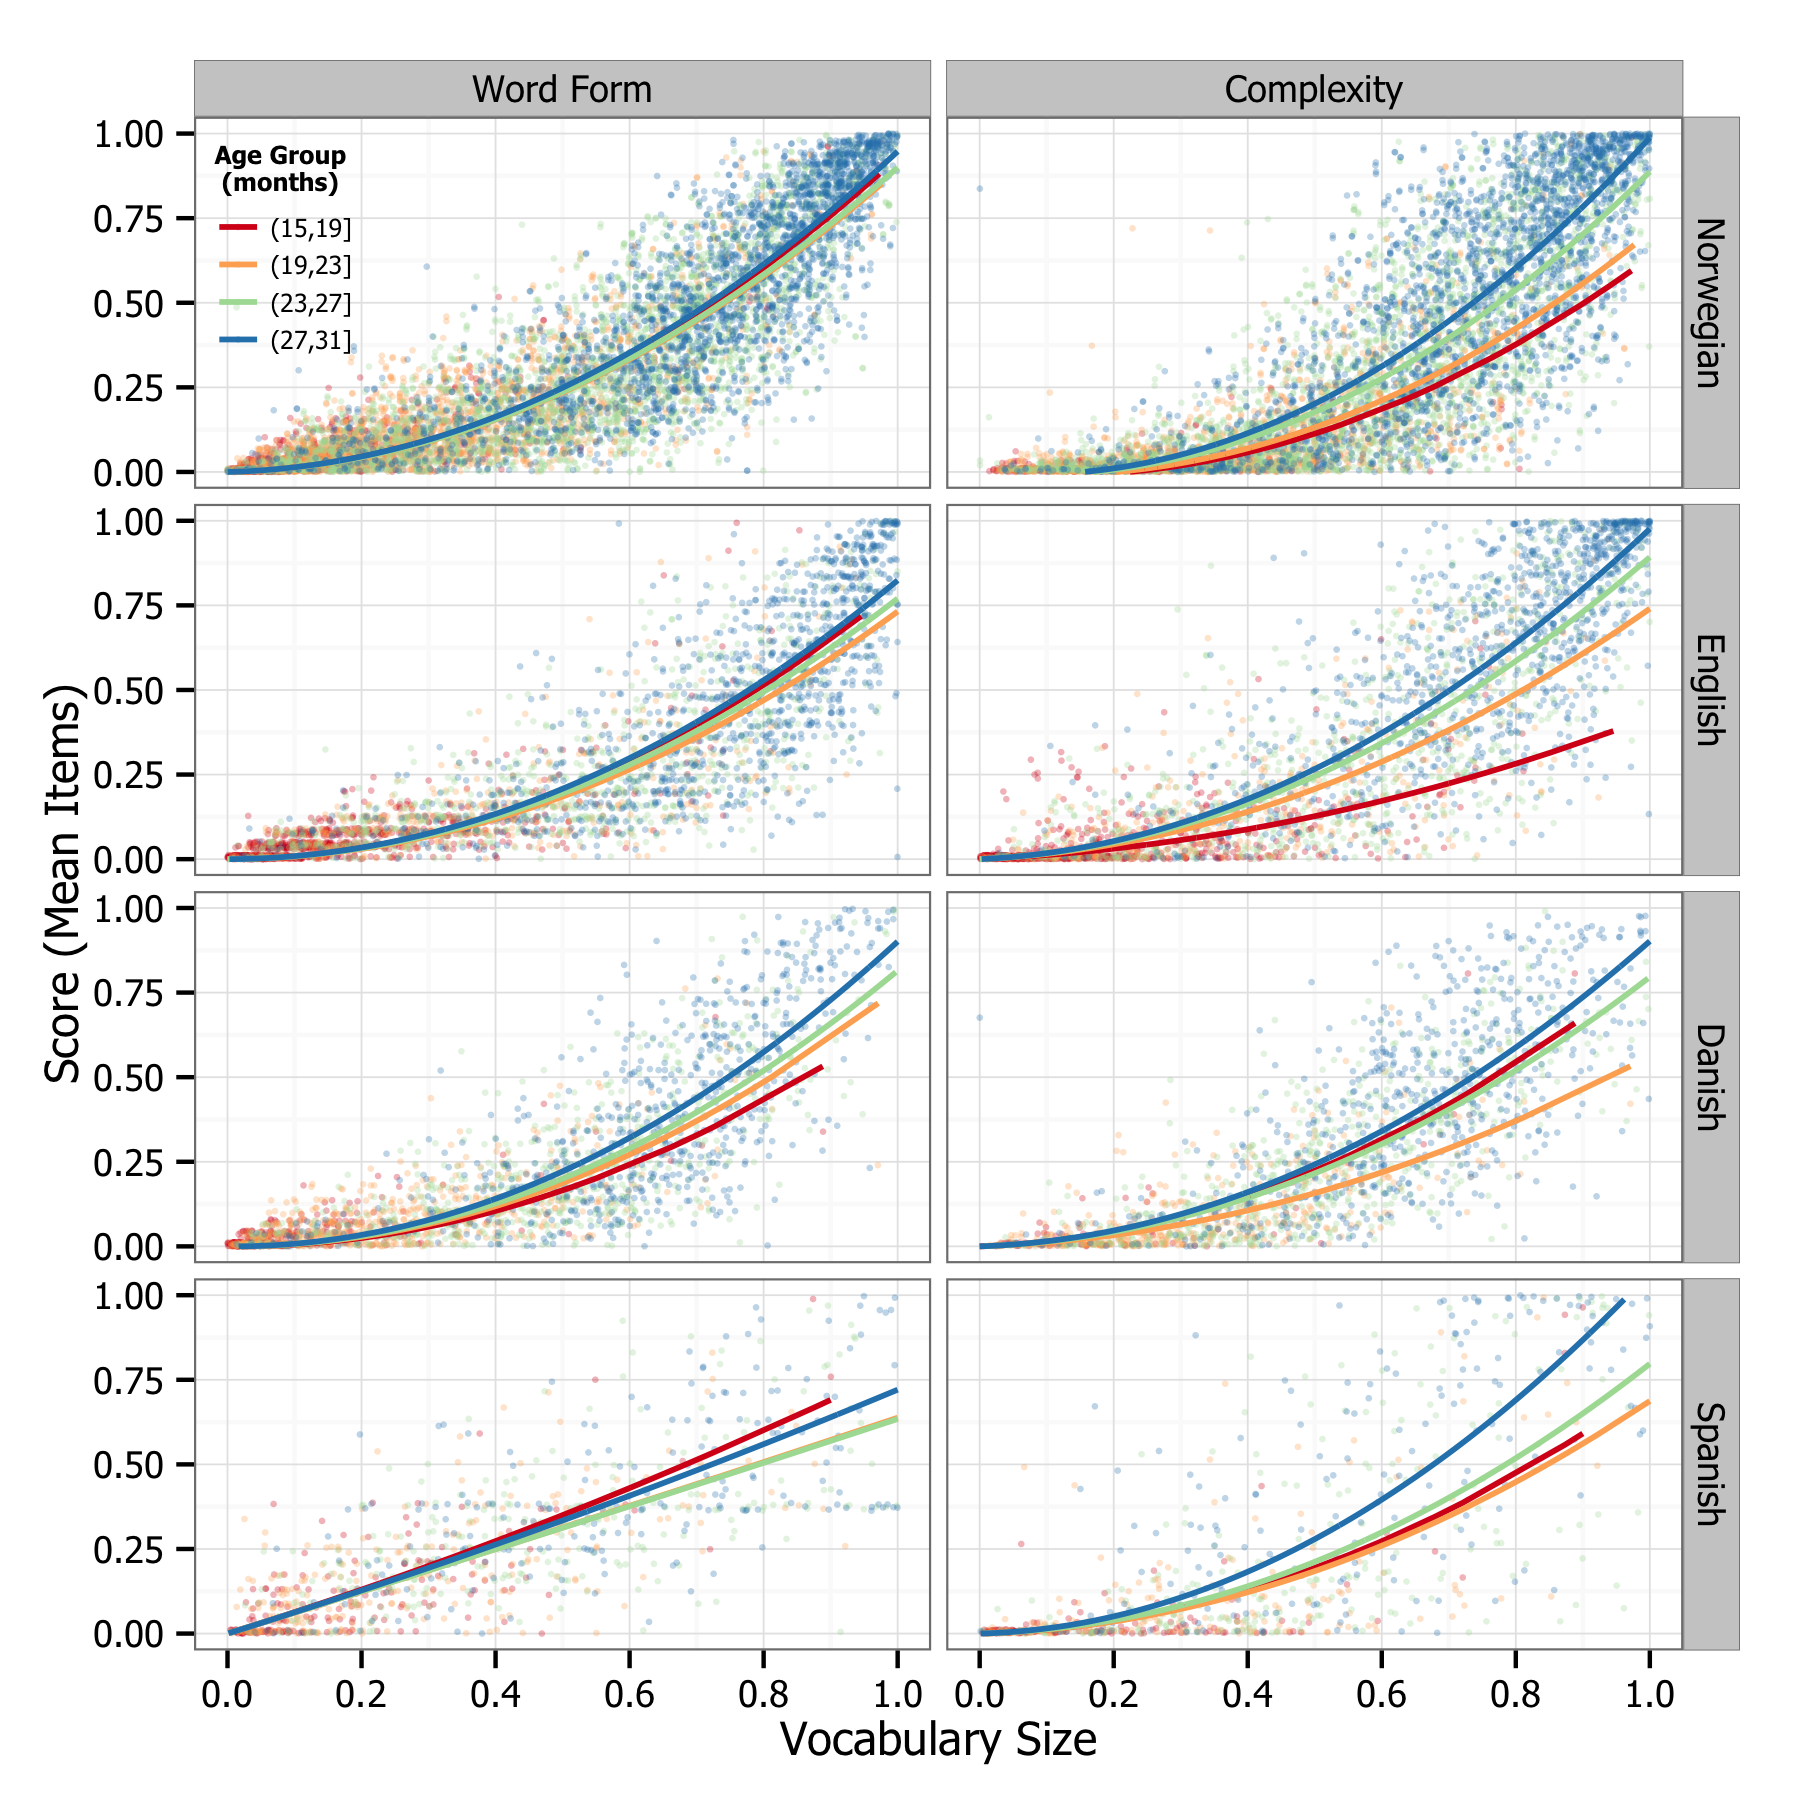
\includegraphics[scale=0.8]{plots/grammar.png}
\end{center}
\caption{Grammar!} 
\label{grammar}
\end{figure*}

[staaaaaaaaats]

\begin{figure}[hbtp]
\begin{center}
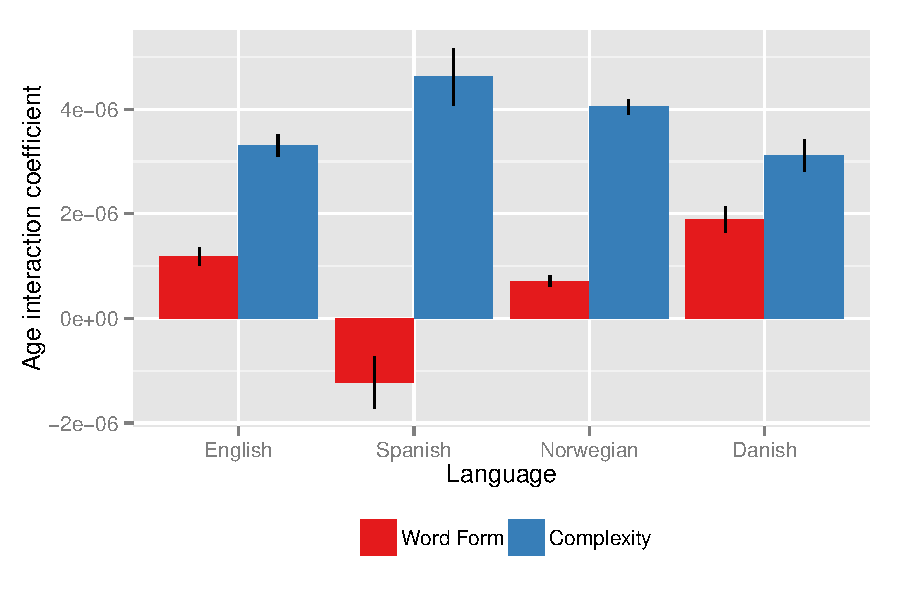
\includegraphics[width=\linewidth]{plots/coeffs}
\end{center}
\caption{Coefficients} 
\label{coeffs}
\end{figure}

[Wrap up aggregate syntax/morphology.]

\clearpage

[Talk about the item-by-item models.]

\begin{figure}[h]
\begin{center}
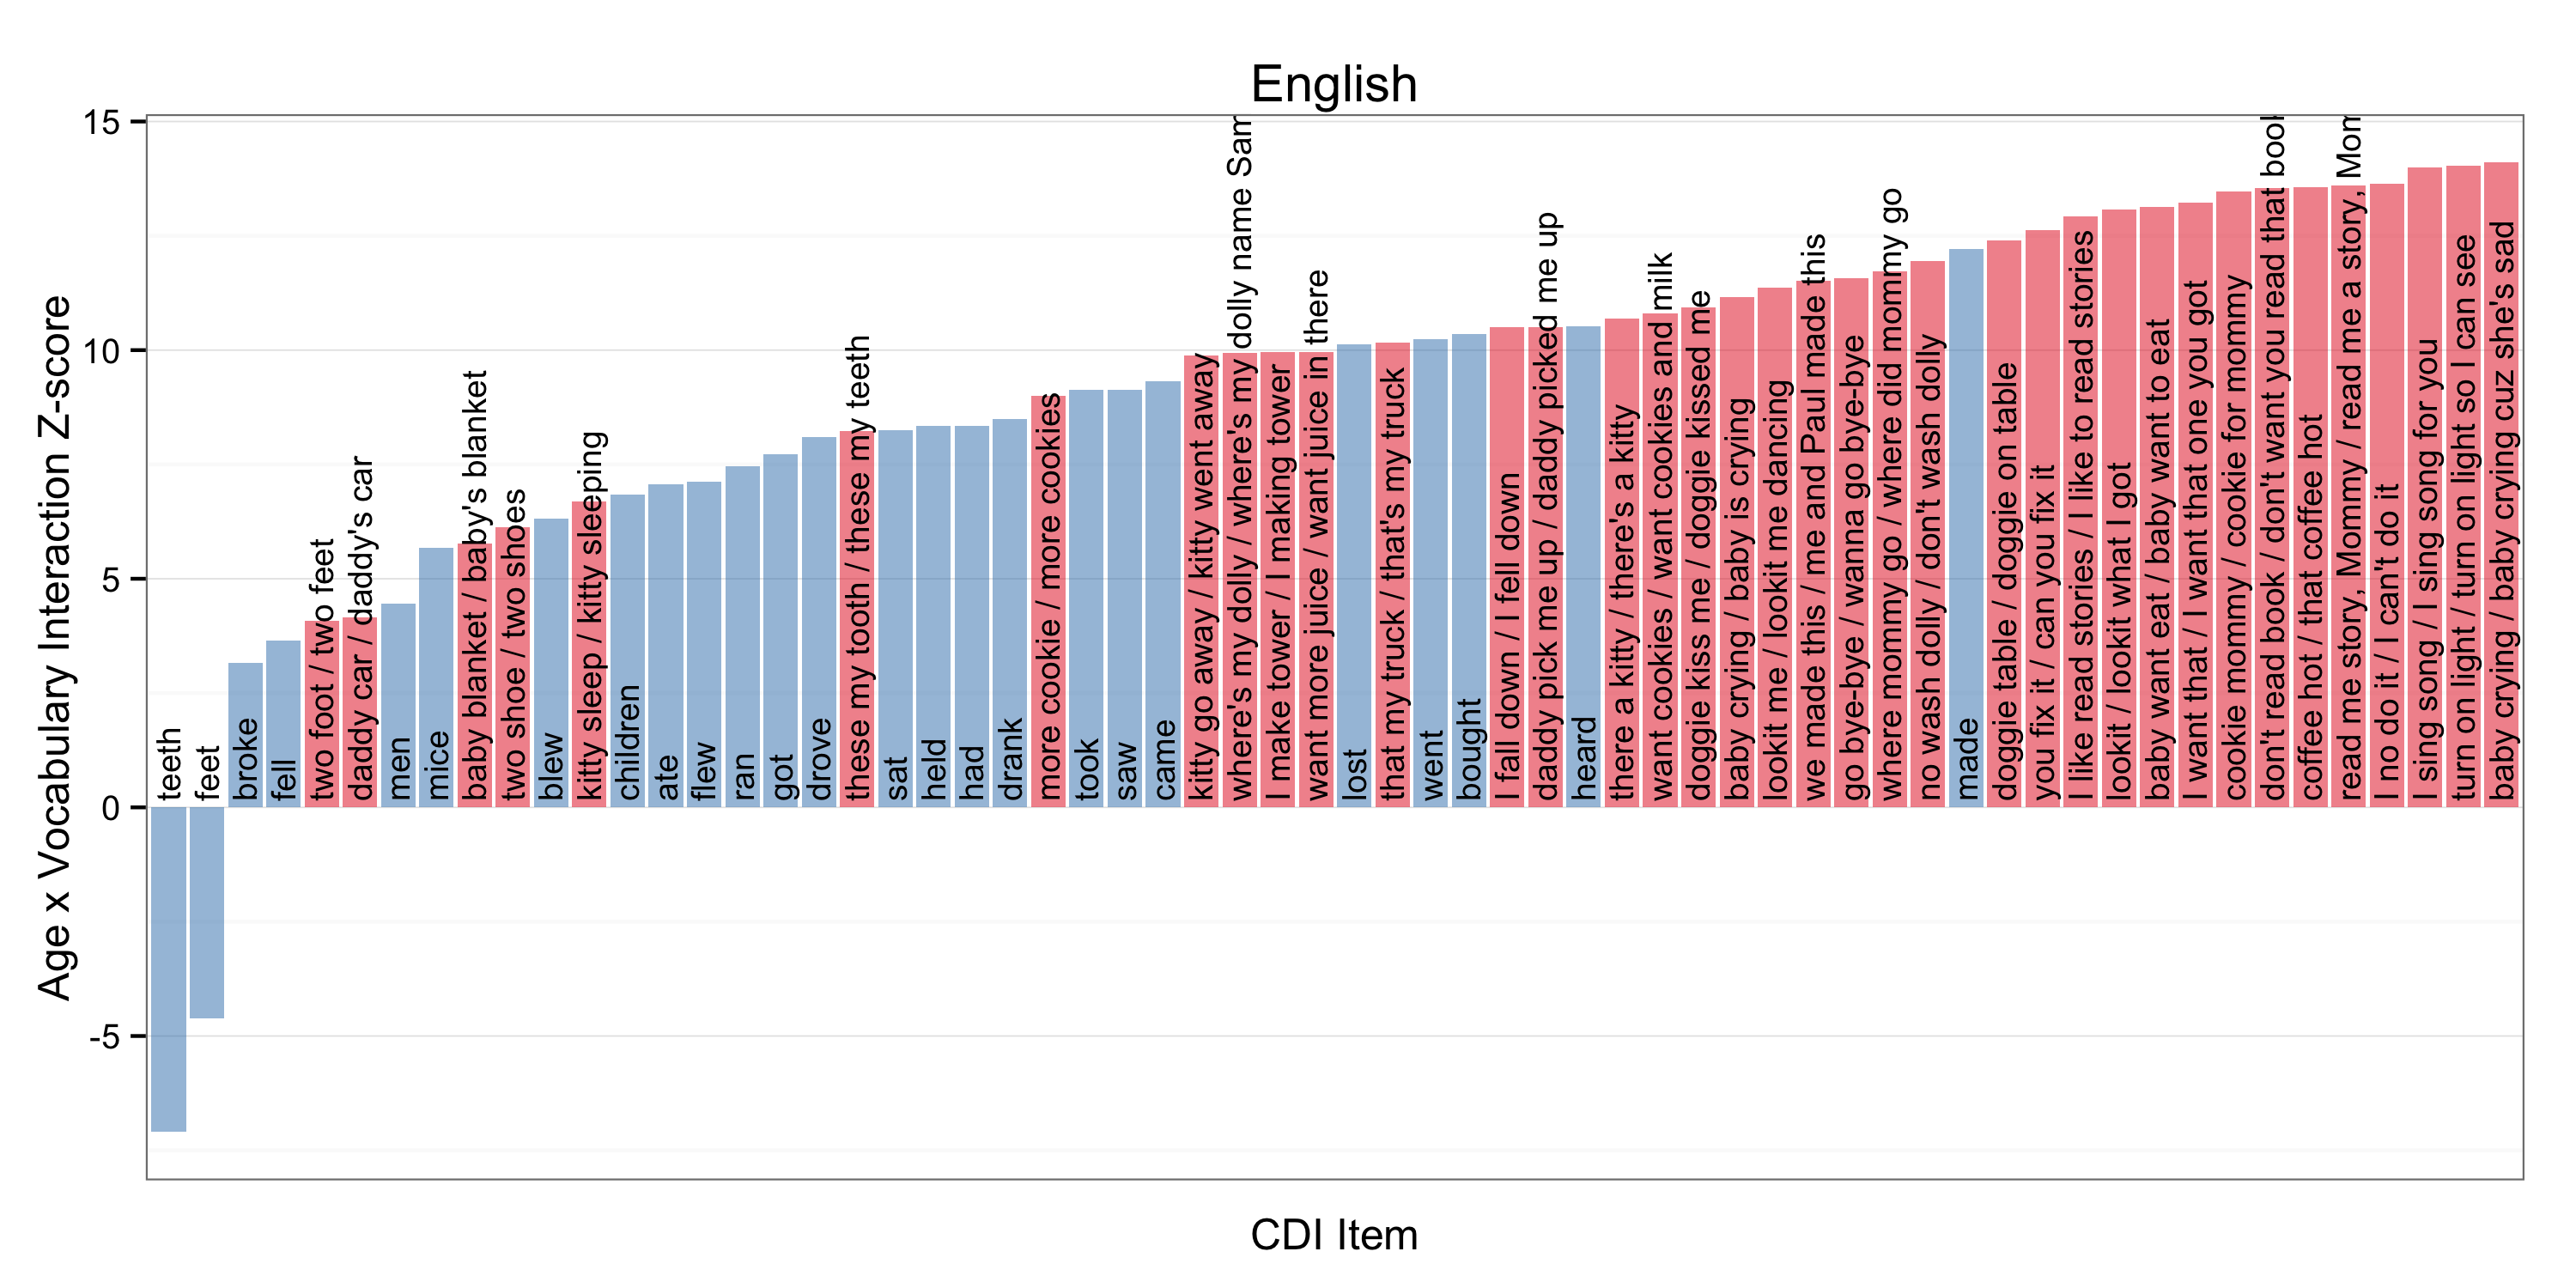
\includegraphics[width=\linewidth]{plots/english_interactions}
\end{center}
\caption{English} 
\label{english_interactions}
\end{figure}

\begin{figure}[h]
\begin{center}
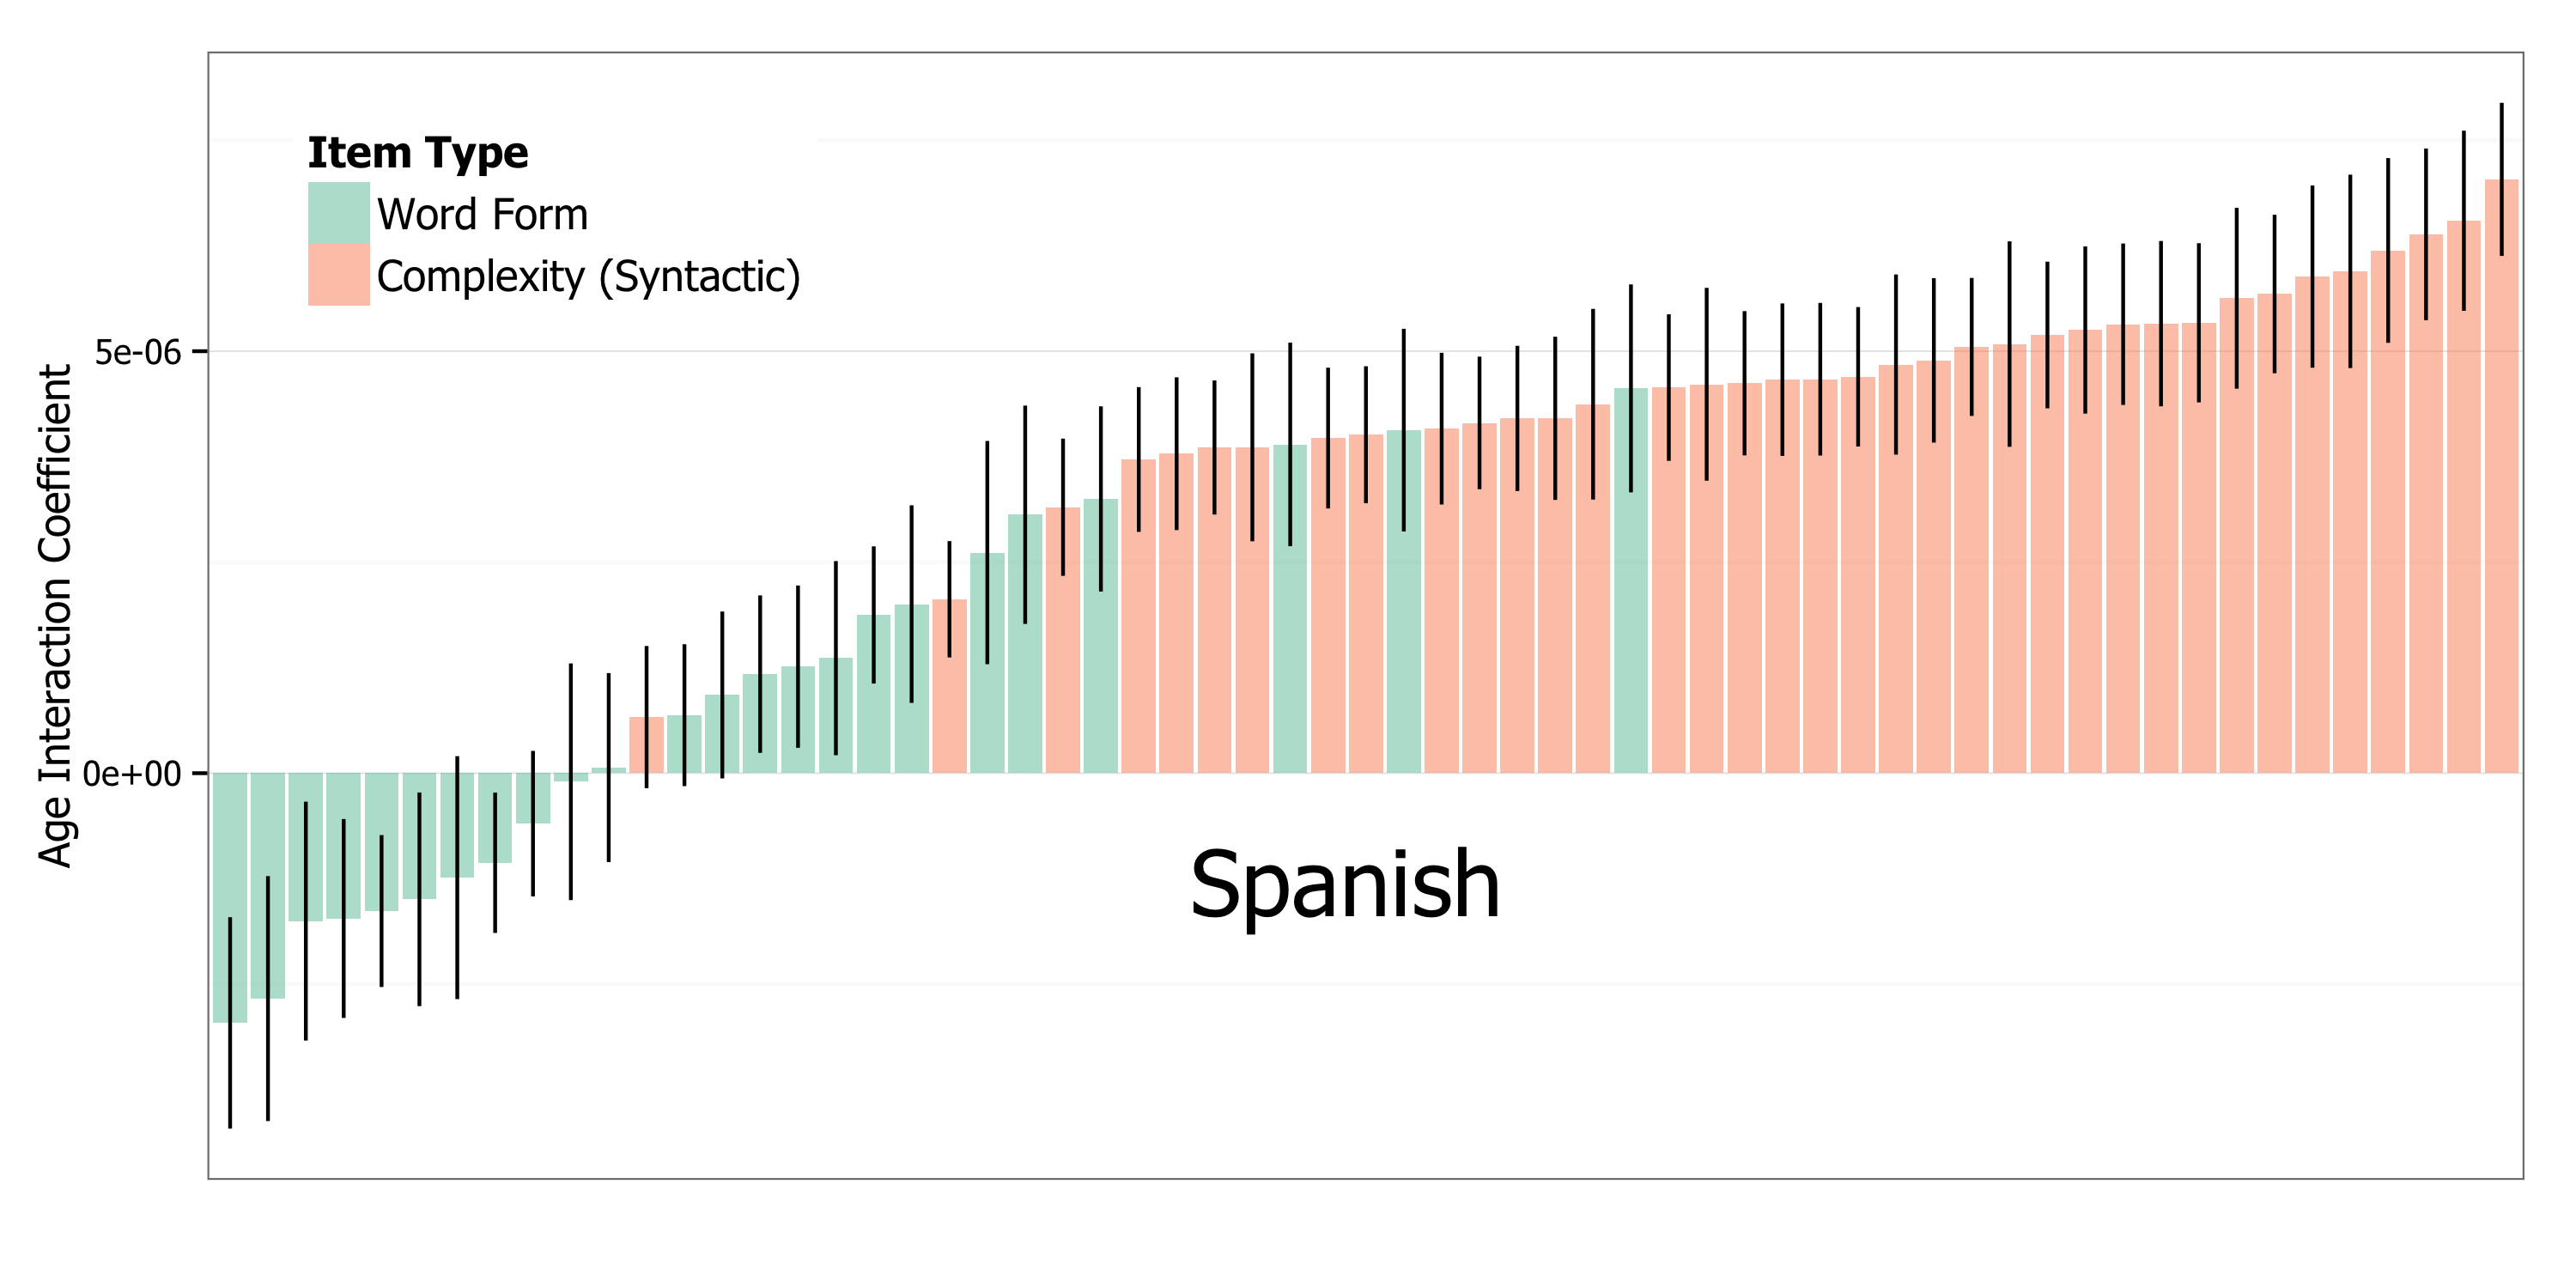
\includegraphics[width=\linewidth]{plots/spanish_interactions}
\end{center}
\caption{Spanish} 
\label{spanish_interactions}
\end{figure}

\begin{figure}[h]
\begin{center}
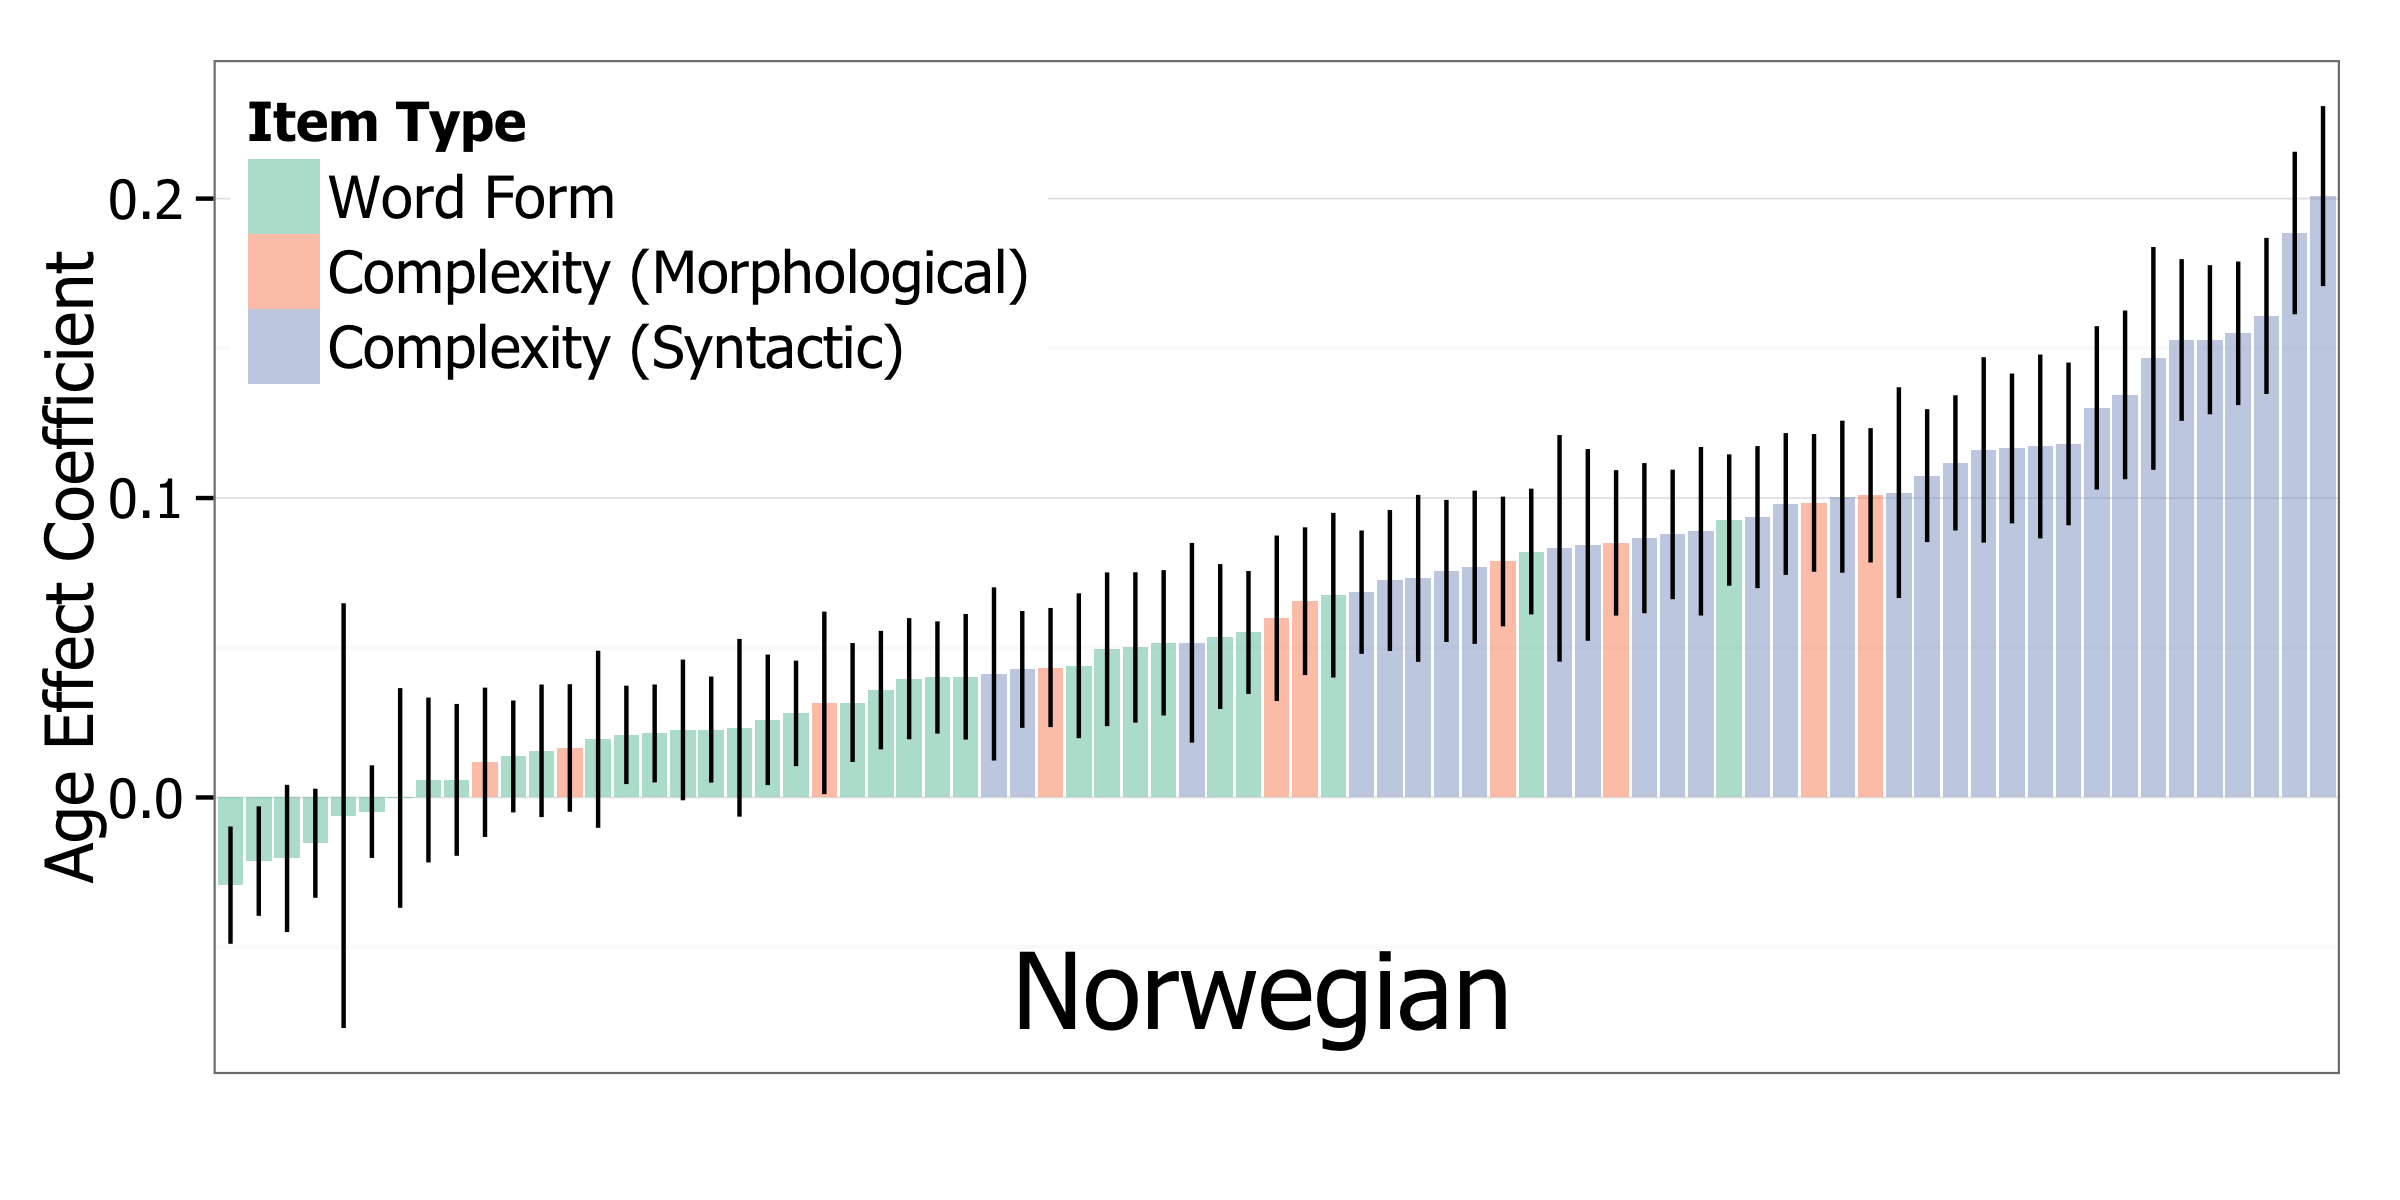
\includegraphics[width=\linewidth]{plots/norwegian_interactions}
\end{center}
\caption{Norwegian} 
\label{norwegian_interactions}
\end{figure}

\begin{figure}[h]
\begin{center}
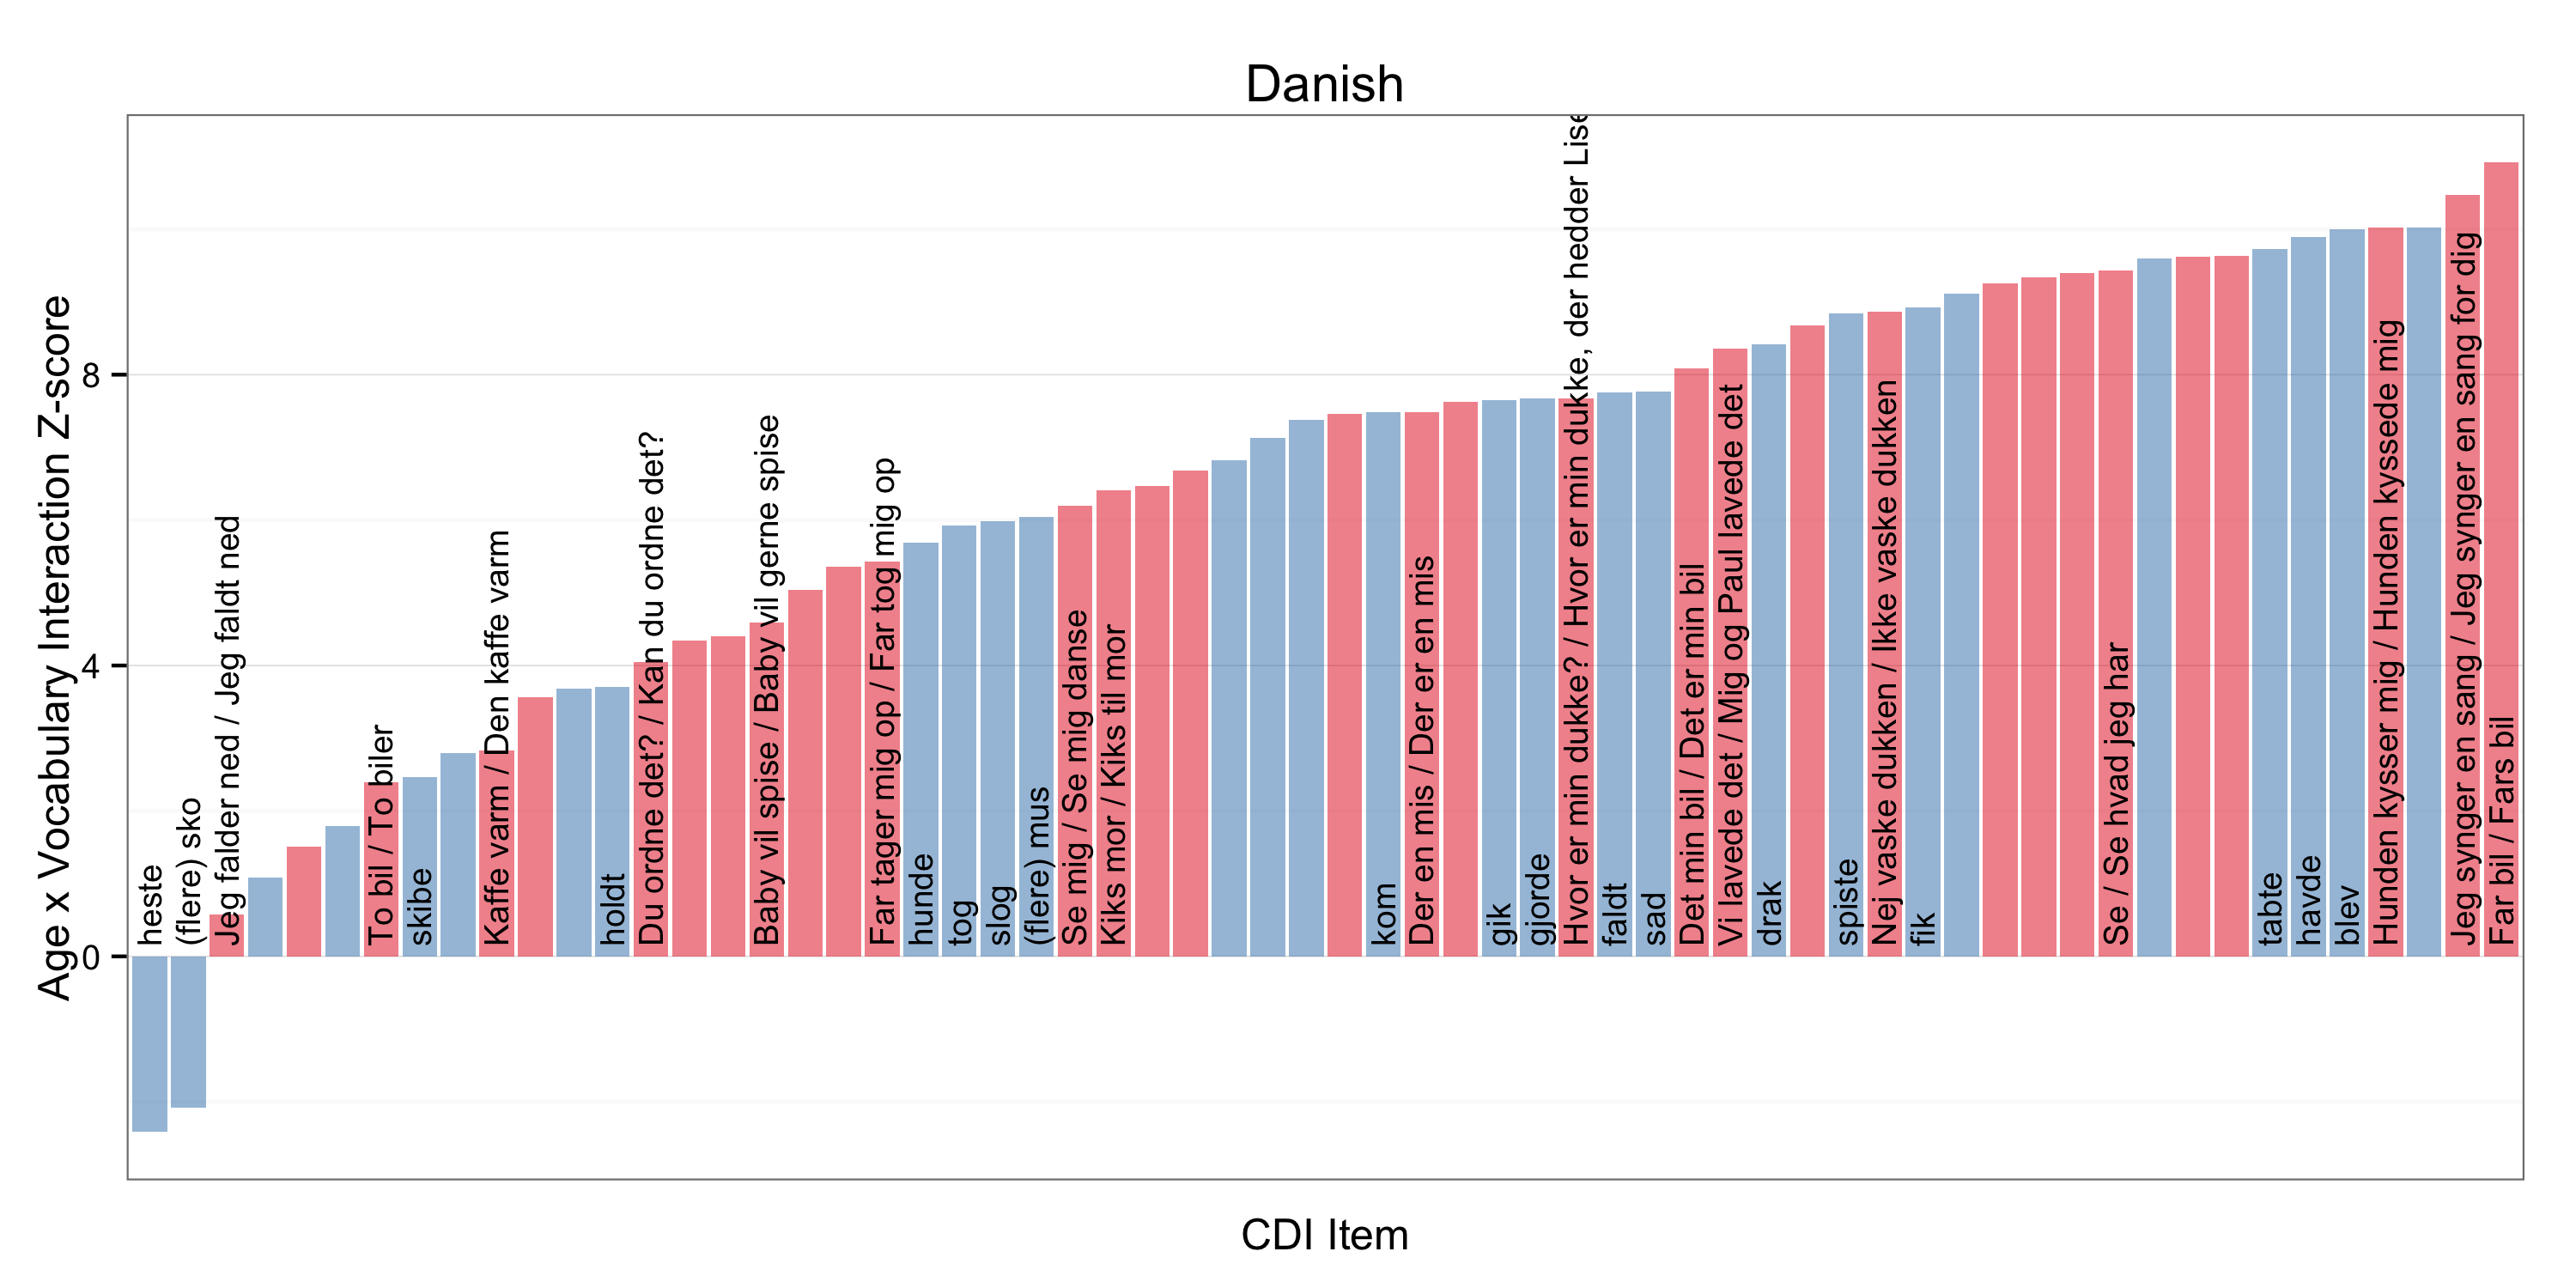
\includegraphics[width=\linewidth]{plots/danish_interactions}
\end{center}
\caption{Danish} 
\label{danish_interactions}
\end{figure}

[Wrap up syntax/morphology.]

\clearpage

\subsection{Lexical Composition}

[Talk about vocab composition results, statistical analyses.]

\begin{figure*}[!ht]
\begin{center}
\includegraphics[scale=1]{plots/composition.png}
\end{center}
\caption{Dat plot though} 
\label{age_composition}
\end{figure*}

\clearpage

\section{Discussion}

\section{Conclusion}

\section{Acknowledgments}

\clearpage

\section{References}

\bibliographystyle{apacite}

\setlength{\bibleftmargin}{.125in}
\setlength{\bibindent}{-\bibleftmargin}

\bibliography{CogSci}


\end{document}
